\documentclass{Configuration_Files/PoliMi3i_thesis}

%------------------------------------------------------------------------------
%	REQUIRED PACKAGES AND  CONFIGURATIONS
%------------------------------------------------------------------------------

% CONFIGURATIONS
\usepackage{parskip} % For paragraph layout
\usepackage{setspace} % For using single or double spacing
\usepackage{emptypage} % To insert empty pages
\usepackage{multicol} % To write in multiple columns (executive summary)
\usepackage{numprint} % Print formatted numbers
\setlength\columnsep{15pt} % Column separation in executive summary
\setlength\parindent{0pt} % Indentation
\usepackage{subfiles} % Include sub files
\usepackage{comment} % Comments
\raggedbottom  

% PACKAGES FOR TITLES
\usepackage{titlesec}
% \titlespacing{\section}{left spacing}{before spacing}{after spacing}
\titlespacing{\section}{0pt}{3.3ex}{2ex}
\titlespacing{\subsection}{0pt}{3.3ex}{1.65ex}
\titlespacing{\subsubsection}{0pt}{3.3ex}{1ex}
\usepackage{color}

% PACKAGES FOR LANGUAGE AND FONT
\usepackage[english]{babel} % The document is in English  
\usepackage[utf8]{inputenc} % UTF8 encoding
\usepackage[T1]{fontenc} % Font encoding
\usepackage[11pt]{moresize} % Big fonts

% PACKAGES FOR IMAGES
\usepackage{graphicx}
\usepackage{transparent} % Enables transparent images
\usepackage{eso-pic} % For the background picture on the title page
\usepackage{subfig} % Numbered and caption subfigures using \subfloat.
\usepackage{tikz} % A package for high-quality hand-made figures.
\usetikzlibrary{}
\graphicspath{{./Images/}} % Directory of the images
\usepackage{caption} % Coloured captions
\usepackage{xcolor} % Coloured captions
\usepackage{amsthm,thmtools,xcolor} % Coloured "Theorem"
\usepackage{float}

% STANDARD MATH PACKAGES
\usepackage{amsmath}
\usepackage{amsthm}
\usepackage{amssymb}
\usepackage{amsfonts}
\usepackage{bm}
\usepackage[overload]{empheq} % For braced-style systems of equations.
\usepackage{fix-cm} % To override original LaTeX restrictions on sizes

% PACKAGES FOR TABLES
\usepackage{tabularx}
\usepackage{longtable} % Tables that can span several pages
\usepackage{colortbl}

% PACKAGES FOR ALGORITHMS (PSEUDO-CODE)
\usepackage{algorithm}
\usepackage{algorithmic}

% PACKAGES FOR REFERENCES & BIBLIOGRAPHY
\usepackage[colorlinks=true,linkcolor=black,anchorcolor=black,citecolor=black,filecolor=black,menucolor=black,runcolor=black,urlcolor=black]{hyperref} % Adds clickable links at references
\usepackage{cleveref}
\usepackage[square, numbers, sort&compress]{natbib} % Square brackets, citing references with numbers, citations sorted by appearance in the text and compressed
\bibliographystyle{abbrvnat} % You may use a different style adapted to your field

% OTHER PACKAGES
\usepackage{pdfpages} % To include a pdf file
\usepackage{afterpage}
\usepackage{lipsum} % DUMMY PACKAGE
\usepackage{fancyhdr} % For the headers
\fancyhf{}

\usepackage{listings} % code snippets
\usepackage{courier}
\lstset{framextopmargin=50pt,frame=bottomline}
\definecolor{mygreen}{rgb}{0,0.6,0}
\definecolor{mygray}{rgb}{0.5,0.5,0.5}
\definecolor{mymauve}{rgb}{0.58,0,0.82}
\lstset{ %
  backgroundcolor=\color{white},   % choose the background color
  basicstyle=\footnotesize\ttfamily,        % size of fonts used for the code
  breaklines=true,                 % automatic line breaking only at whitespace
  captionpos=b,                    % sets the caption-position to bottom
  commentstyle=\color{mygreen},    % comment style
  escapeinside={\%*}{*)},          % if you want to add LaTeX within your code
  keywordstyle=\color{blue},       % keyword style
  stringstyle=\color{mymauve},     % string literal style
  frame=none                       % no lower frame
}

% Input of configuration file. Do not change config.tex file unless you really know what you are doing. 
% Define blue color typical of polimi
\definecolor{bluepoli}{cmyk}{0.4,0.1,0,0.4}
\definecolor{green}{cmyk}{1,0,0.5703,0.4980}

% Custom theorem environments
\declaretheoremstyle[
  headfont=\color{bluepoli}\normalfont\bfseries,
  bodyfont=\color{black}\normalfont\itshape,
]{colored}

% Set-up caption colors
\captionsetup[figure]{labelfont={color=bluepoli}} % Set colour of the captions
\captionsetup[table]{labelfont={color=bluepoli}} % Set colour of the captions
\captionsetup[algorithm]{labelfont={color=bluepoli}} % Set colour of the captions

\theoremstyle{colored}
\newtheorem{theorem}{Theorem}[chapter]
\newtheorem{proposition}{Proposition}[chapter]

% Enhances the features of the standard "table" and "tabular" environments.
\newcommand\T{\rule{0pt}{2.6ex}}
\newcommand\B{\rule[-1.2ex]{0pt}{0pt}}

% Pseudo-code algorithm descriptions.
\newcounter{algsubstate}
\renewcommand{\thealgsubstate}{\alph{algsubstate}}
\newenvironment{algsubstates}
  {\setcounter{algsubstate}{0}%
   \renewcommand{\STATE}{%
     \stepcounter{algsubstate}%
     \Statex {\small\thealgsubstate:}\space}}
  {}

% New font size
\newcommand\numfontsize{\@setfontsize\Huge{200}{60}}

% Title format: chapter
\titleformat{\chapter}[hang]{
\fontsize{50}{20}\selectfont\bfseries\filright}{\textcolor{bluepoli} \thechapter\hsp\hspace{2mm}\textcolor{bluepoli}{|   }\hsp}{0pt}{\huge\bfseries \textcolor{bluepoli}
}

% Title format: section
\titleformat{\section}
{\color{bluepoli}\normalfont\Large\bfseries}
{\color{bluepoli}\thesection.}{1em}{}

% Title format: subsection
\titleformat{\subsection}
{\color{bluepoli}\normalfont\large\bfseries}
{\color{bluepoli}\thesubsection.}{1em}{}

% Title format: subsubsection
\titleformat{\subsubsection}
{\color{bluepoli}\normalfont\large\bfseries}
{\color{bluepoli}\thesubsubsection.}{1em}{}

% Shortening for setting no horizontal-spacing
\newcommand{\hsp}{\hspace{0pt}}

\makeatletter
% Renewcommand: cleardoublepage including the background pic
\renewcommand*\cleardoublepage{%
  \clearpage\if@twoside\ifodd\c@page\else
  \null
  \AddToShipoutPicture*{\BackgroundPic}
  \thispagestyle{empty}%
  \newpage
  \if@twocolumn\hbox{}\newpage\fi\fi\fi}
\makeatother

%For correctly numbering algorithms
\numberwithin{algorithm}{chapter}

%----------------------------------------------------------------------------
%	NEW COMMANDS DEFINED
%----------------------------------------------------------------------------

% EXAMPLES OF NEW COMMANDS
\newcommand{\bea}{\begin{eqnarray}} % Shortcut for equation arrays
\newcommand{\eea}{\end{eqnarray}}
\newcommand{\e}[1]{\times 10^{#1}}  % Powers of 10 notation

%----------------------------------------------------------------------------
%	ADD YOUR PACKAGES (be careful of package interaction)
%----------------------------------------------------------------------------

%----------------------------------------------------------------------------
%	ADD YOUR DEFINITIONS AND COMMANDS (be careful of existing commands)
%----------------------------------------------------------------------------

%----------------------------------------------------------------------------
%	BEGIN OF YOUR DOCUMENT
%----------------------------------------------------------------------------

\begin{document}

\fancypagestyle{plain}{%
\fancyhf{} % Clear all header and footer fields
\fancyhead[RO,RE]{\thepage} %RO=right odd, RE=right even
\renewcommand{\headrulewidth}{0pt}
\renewcommand{\footrulewidth}{0pt}}

%----------------------------------------------------------------------------
%	TITLE PAGE
%----------------------------------------------------------------------------

\pagestyle{empty} % No page numbers
\frontmatter % Use roman page numbering style (i, ii, iii, iv...) for the preamble pages

\puttitle{
	title=Titolo da scegliere, % Title of the thesis
	name=Ciriello Giovanni, % Author Name and Surname
	course=ICT Engineering\, Business and Innovation - Computer Science Engineering, % Study Programme (in Italian)
	ID  = 963100,  % Student ID number (numero di matricola)
	advisor= Prof. Francalanci Chiara, % Supervisor name
	coadvisor={Ravanelli Paolo}, % Co-Supervisor name, remove this line if there is none
	academicyear={2021-22},  % Academic Year
} % These info will be put into your Title page 

%----------------------------------------------------------------------------
%	PREAMBLE PAGES: ABSTRACT (inglese e italiano), EXECUTIVE SUMMARY
%----------------------------------------------------------------------------
\startpreamble
\setcounter{page}{1} % Set page counter to 1

% ABSTRACT IN ENGLISH
\chapter*{Abstract} 
Here goes the Abstract in English of your thesis followed by a list of keywords.
The Abstract is a concise summary of the content of the thesis (single page of text)
and a guide to the most important contributions included in your thesis.
The Abstract is the very last thing you write.
It should be a self-contained text and should be clear to someone who hasn't (yet) read the whole manuscript.
The Abstract should contain the answers to the main scientific questions that have been addressed in your thesis.
It needs to summarize the adopted motivations and the adopted methodological approach as well as the findings of your work and their relevance and impact.
The Abstract is the part appearing in the record of your thesis inside POLITesi,
the Digital Archive of PhD and Master Theses (Laurea Magistrale) of Politecnico di Milano.
The Abstract will be followed by a list of four to six keywords.
Keywords are a tool to help indexers and search engines to find relevant documents.
To be relevant and effective, keywords must be chosen carefully.
They should represent the content of your work and be specific to your field or sub-field.
Keywords may be a single word or two to four words. 
\\
\\
\textbf{Keywords:} here, the keywords, of your thesis % Keywords

% ABSTRACT IN ITALIAN
\chapter*{Abstract in lingua italiana}

Il trasporto marittimo è storicamente considerato il mezzo più efficace e diffuso per trasferire su lunga distanza consistenti carichi di merci in termini di dimensione e peso. Costituendo la base del 90\% del commercio mondiale \cite{trasporto-marittimo}, la sicurezza rappresenta uno degli aspetti più discussi e una intensa attività di ricerca ha interessato questo campo negli ultimi tempi.  
In tale contesto, sempre più enti stanno implementando algoritmi di controllo che sfruttano tecniche di intelligenza artificiale e machine learning al fine di monitorare i viaggi marittimi. ARCOS (Arctic Observatory for Copernicus SEA) è un progetto finanziato dall'Unione Europea che ha, tra i suoi obiettivi, quello di sviluppare sistemi di allerta predittiva in grado di fornire un continuo monitoraggio della regione Artica. A tale scopo, ha collezionato dati relativi ai tragitti percorsi nella zona interessata da mezzi di trasporto marittimo. Tali dati contengono messaggi che rispettano lo standard AIS (Automatic Identification System), cruciale per garantire la sicurezza delle operazioni marittime. Il suo funzionamento si basa su numerosi sensori presenti a bordo e una ricetrasmittente che invia i dati - con una frequenza dell’ordine di minuti - a satelliti in orbita (messaggi S-AIS). Lo scopo della tesi è quello di proporre una metodologia per rilevare anomalie di qualsiasi genere a partire da un dataset di messaggi AIS. Al fine di raggiungere tale obiettivo, i messaggi sono stati in primo luogo raggruppati in tragitti, che rappresentano l'entità sulla quale si è scelto di rilevare anomalie. Su di essi è stato applicato un algoritmo di clustering basato su densità spaziale (DBSCAN) e successivamente tecniche di analisi dei valori anomali risultanti al fine di valutarne la rilevanza e il significato. Il metodo è stato validato su un dataset di testing, contenente più di 95 milioni di messaggi, sul quale sono state rilevate potenziali anomalie relative a distanza percorsa, tempi di navigazione e variazioni del carico. Un possibile sviluppo futuro è la creazione di un sistema di allerta predittiva che - sfruttando la metodologia proposta - permetta ai satelliti il rilevamento di anomalie in fase di ricezione dei messaggi come step preliminare ad un controllo manuale da parte delle autorità competenti.

\\
\\
\textbf{Parole chiave:} AIS, Anomalia. Trasporto marittimo, DBSCAN, monitoraggio

%----------------------------------------------------------------------------
%	LIST OF CONTENTS/FIGURES/TABLES/SYMBOLS
%----------------------------------------------------------------------------

% TABLE OF CONTENTS
\thispagestyle{empty}
\tableofcontents % Table of contents 
\thispagestyle{empty}
\cleardoublepage

%-------------------------------------------------------------------------
%	THESIS MAIN TEXT
%-------------------------------------------------------------------------
% In the main text of your thesis you can write the chapters in two different ways:
%
%(1) As presented in this template you can write:
%    \chapter{Title of the chapter}
%    *body of the chapter*
%
%(2) You can write your chapter in a separated .tex file and then include it in the main file with the following command:
%    \chapter{Title of the chapter}
%    \input{chapter_file.tex}
%
% Especially for long thesis, we recommend you the second option.

\addtocontents{toc}{\vspace{2em}} % Add a gap in the Contents, for aesthetics
\mainmatter % Begin numeric (1,2,3...) page numbering

% --------------------------------------------------------------------------
% NUMBERED CHAPTERS % Regular chapters following
% --------------------------------------------------------------------------

\chapter*{Introduction}
\label{ch:introduction}

Il lavoro presentato in questo documento è collegato al progetto ARCOS e ha come obiettivo la rilevazione di potenziali anomalie nei tragitti effettuati da mezzi di trasporto marittimi nella zona dell'Artico.

Nel capitolo \ref{ch:stateOfTheArt} si fa una panoramica del contesto riguardante il progetto ARCOS e i suoi obiettivi, si descrive lo standard di messaggi marittimi AIS con un focus sui messaggi satellitari (S-AIS), e anche una descrizione delle tecniche di anomaly detection attualmente utilizzate, con un focus sul DBSCAN, che verrà utilizzato per clusterizzare i viaggi.

Il capitolo \ref{ch:methodology} include la completa metologia utilizzata, partendo dai dati AIS grezzi, iniziando con tecniche di data cleaning e procedendo con la generazione delle entitià tragitti tramite un algoritmo di raggruppamento logico. Procedendo ulteriormente con la selezione e la computazione delle feature dei viaggi da analizzare (features engineering) e l'implementazione dell'algoritmo di clustering DBSCAN. Infine la metodologia comprende tecniche di data analysis utili a comprendere i motivi per cui alcuni viaggi sono considerati outlier e quali sono significativi o meno.

Nel capitolo \ref{ch:testing} si descrivono i risultati ottenuti con un dataset contenente più di 95 milioni di messaggi cercando di dare un'interpretazione alle anomalie più rilevanti.


\chapter{State of the Art}

\section{The context}

    \subsection{The ARCOS Project}
    \textbf{ARCOS} (ARCtic Observatory for Copernicus SEA Security Service) is an EU-funded project (specifically from the \textit{European Union’s Horizon 2020 research and innovation programme}) whose goal is to design and implement an early warning system that provides continuous monitoring of the \textbf{Arctic region} \cite{arcos}. 
    
    Designed to create actionable security products by processing and merging multi-sensor data, the ARCOS system integrates information available space, non-space sources and products available from Copernicus Services \cite{copernicus}. 
    
    The project system ARCOS handle information at three different levels of scale and user interaction:
    
    \begin{enumerate}
    \item \textbf{Automatic early-warning system}: Integration of multi-channel data sources with the goal of triggering alerts in the region when certain conditions are met. Automatic early warnings are generated when anomalous behaviours are detected, such as the discovery of suspicious targets or large-scale exploitation of natural resources.
    
    \item \textbf{User Driven Alert System} by providing user guidance on the specific location and type of observation objects desired, alarms can be configured based on more specific information, such as activity patterns.
    
    \item \textbf{Geospatial Intelligence Products}. Thanks to the warnings previously generated, geospatial intelligence products requiring human intervention are provided at the user's request. These products require extensive contextual analysis, typically requiring coordinated action at more than one location.
    \end{enumerate}
    
    \begin{figure}[H]
        \centering
        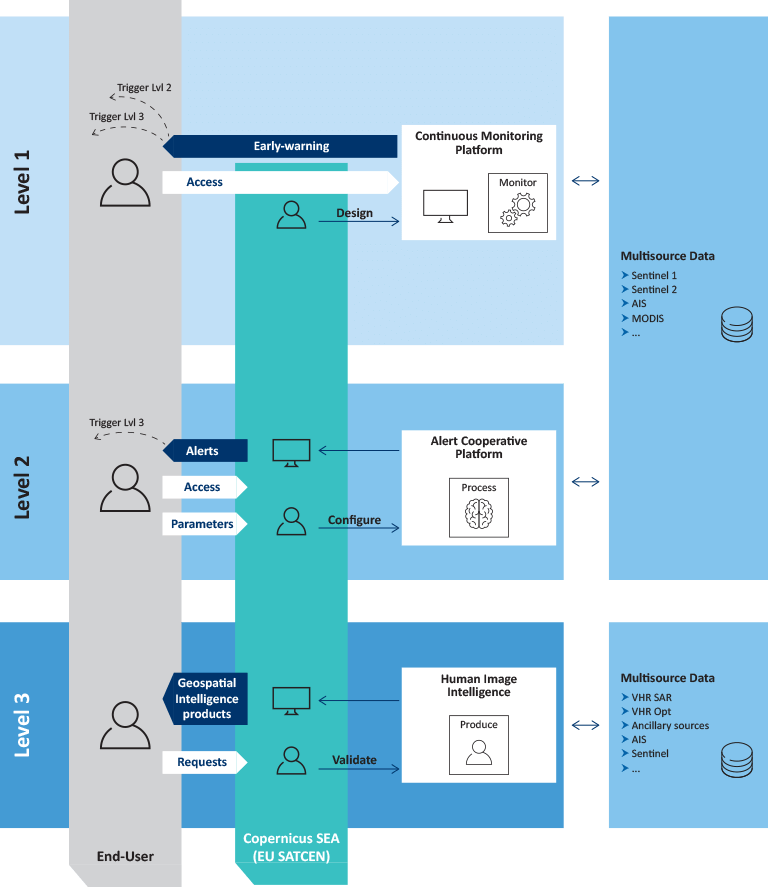
\includegraphics[width=13cm]{Images/1/arcos-design.png}
        \caption{ARCOS Project platform design \cite{arcos}}
    \end{figure}
        

    
\newpage
\section{The AIS Data}
    \subsection{Introduction}
    The \textit{\textbf{Automatic Identification System}} (AIS) is an automatic tracking system widely used by \textit{Vessel Traffic Services} (VTS). AIS is crucial in order to grant safety and security in maritime operations.
    It bases its operation on a transceiver on ships that sends data to others receivers or to satellites.
    
    AIS information includes a variety of data regarding the real-time status of a ship during a voyage, e.g. its unique identifier, position, ship status, and speed. This information is very useful when displayed on the screen of a \textit{Electronic Chart Display and Information System} (ECDIS).
    
    The \textit{International Maritime Organization} (IMO) requires AIS system to be installed on board ships of 300 gross tonnage (i.e. a nonlinear measure of a ship's overall internal volume) or more, cargo ships of 500 gross tonnage and all passenger ships, regardless of size \cite{ais_regulations}.
    
    According to the current regulations AIS systems should:
    \begin{itemize}
        \item Automatically relay information - including vessel identity, type, position, course, speed, navigational status, and other safety-related information
        \item Automatically receive such information from similarly equipped vessels; 
        \item Monitor and track ships;
        \item Exchange data with coast facilities.
    \end{itemize}

    Despite the strict regulations in place on AIS systems, for a variety of reasons, ships may turn off their AIS transceivers or, much more frequently, technical errors may occur that affect the continuity of the reception of AIS messages.
    
    \subsection{A focus on Satellite AIS}
    AIS is designed to assist a ship's watch-keeping officers and to enable maritime authorities to track and monitor ship movements. AIS integrates a standardized VHF (Very High Frequency) transceiver with a positioning system, with other electronic navigation sensors, such as a gyrocompass or rate-of-turn indicator. Vessels equipped with AIS transceivers can be tracked by AIS base stations along coastlines or, when out of range of terrestrial networks, via a high number of satellites equipped with specialized AIS receivers. 
    \\
    Satellite Automatic Identification System (\textbf{S-AIS}) is based on satellite infrastructure and in particular on satellites in Low Earth Orbit (LEO). These satellites are equipped with AIS receivers and the received messages are retransmitted in a broadcast system.
    The just described technical solution increases the range of AIS and makes it possible to cover an area between 2\% and 4\% of the Earth's surface with a LEO satellite. \cite{dbscan_ais}.
    
    The main problem posed by S-AIS is the collision of data packets: If a large number of ships use the same transmission time slot, the satellite component receiving the AIS messages might have problems correctly identifying the packet affiliation.
    \\
    The main reason for this is that S-AIS operates in a larger area covering a wide area, and therefore collects signals from multiple transmitters, resulting in collisions of data packets.
    As a result, data belonging to different packets get mixed and it is not possible to recover the packet in its original form. As a result, important parts of messages from AIS are lost, so a considerable number of messages are not recognised and forwarded to a terrestrial part of the system. As a result, it is not possible to monitor part of the trajectory of ships \cite{dbscan_ais}.
    
    % https://en.wikipedia.org/wiki/Automatic_identification_system#cite_note-1:~:text=External%20links-,Viewing%20and%20using%20AIS%20data,-%5Bedit%5D
    
    
\clearpage  

\section{Anomaly Detection Techniques}

    \textbf{Anomaly detection} is a branch in data mining that identifies event or observations that deviate from the normal behavior of a data set \cite{anomaly_detection}. Anomaly detection is applicable in a very large number and variety of domains and that makes it so widely used.
    \\
    Anomalous data can indicate critical incidents, such as a technical malfunction, or potential opportunities, such as changing consumer behavior. Machine learning techniques are increasingly being used to automate anomaly detection.
    
    \subsection{Time Series}
    The starting point for a well-functioning anomaly detection algorithm is the analysis of time series.
    \\
    Time series are sequences of values over time. This means that each entry in the data set can be viewed as a pair of two elements: a timestamp for when the metric was measured, and the set of values associated with that metric at that time. 
    \\ 
    Time series data should not be viewed as a projection of the data set; rather, it contains the information necessary to make fairly accurate guesses about what to expect in the future. Anomaly detection systems use these expectations to identify actionable signals in your data and detect outliers that indicate certain relevant events in your business.
    
    \subsubsection{Time Series in Maritime field}
    In the maritime application domain of anomaly detection, the just mentioned time series are sequences of AIS messages containing the whole set of various parameters representing the state of the ship, i.e. real-time information collected on board a ship by numerous sensors (such as GPS locator, accelerometer, gyroscope, etc.). 
    In S-AIS (Satellite AIS) data, messages are sent to satellites at an average frequency of thirty seconds, but this can be varied depending on ship speed or base station instructions. 
    \\
    The described time series represent the trajectories of the ships, each of them could be defined as a finite sequence of positions of the ship received in chronological order. The problem of packet collisions mentioned leads to a lack of data in the sequence. Thus, such a data point corresponds to a multi-dimensional feature vector of the moving ship at a particular time, and the packet collision problem introduces noise or lack of data.

    \subsection{Clustering Techniques Overview}
    In the field of data analysis, the general task of dividing data points into groups such that the data points in the same groups are more similar to other data points in the same group than those in other groups is called \textbf{clustering} \cite{clustering}.
    \\
    As first important classification, clustering is defined:
    
    \begin{itemize}
    \item \textbf{Hard Clustering} when each data point either belongs entirely to a cluster or does not.
    \item \textbf{Soft Clustering} each data point is not placed in a separate cluster, but is assigned a probability of being included in those clusters.
    \end{itemize}
    \\
    
    \begin{figure}[H]
        \centering
        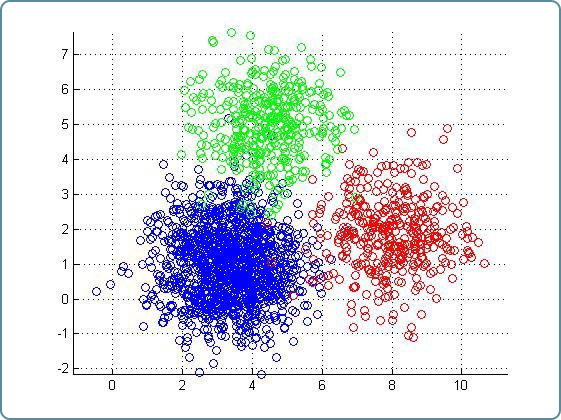
\includegraphics[width=9cm]{Images/1/clustering.png}
        \caption{Visualization of hard clustering technique}
    \end{figure}
        
    
    A basic example of a clustering model is \textbf{K-means}. It comes from the family of \textit{Centroid models} and aims to iteratively partition n data points into k clusters in which each observation belongs to the cluster with the closest mean.
    Its clustering process can be summarized in 5 points:
    
    \begin{enumerate}
        \item Specify the desired number of clusters K;
        \item Randomly assign each data point to a cluster;
        \item Calculate the centres for each cluster;
        \item Re-assign each point to the nearest cluster centre;
        \item Recalculate the cluster centroids;
        \item Repeat steps 4 and 5 until no more improvements are possible.
    \end{enumerate}
    
    \begin{figure}[H]
        \centering
        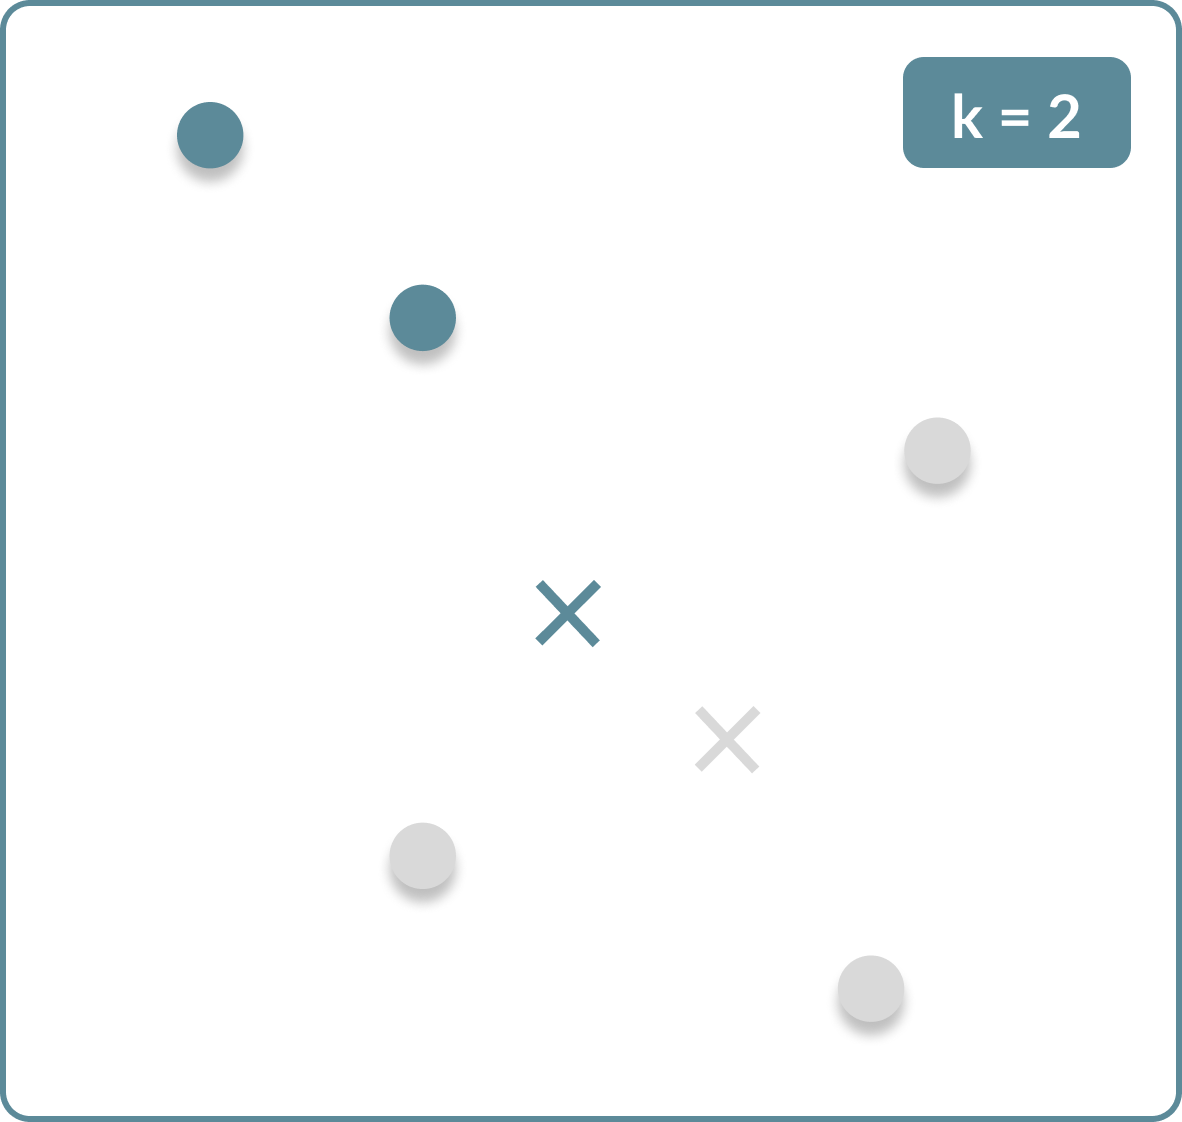
\includegraphics[width=9cm]{Images/1/kmeans.png}
        \caption{Data points and centroids in k-means clustering}
    \end{figure}
    
    There are more than 100 known clustering algorithms, and each method follows a different set of rules for defining similarity between data points. But the class of clustering algorithms that is highlighted in this work is \textbf{density-based clustering algorithms}. These models search the data space for regions of varying density of data points in the data space. It isolates different regions of varying density and assigns the data points within those regions to the same cluster. Popular examples of density models include DBSCAN and OPTICS.
    
    
    \subsection{DBSCAN}
    \textbf{Density-based spatial clustering of Applications with Noise} (DBSCAN) is an algorithm for clustering data based on density.
    \\
    The algorithm works with a given set of points in a given space, it groups the points that are close enough to each other and labels the points that are in low-density regions alone as outliers. DBSCAN is one of the most common clustering algorithms and is also one of the most cited in the scientific literature.
    \\
    In order to represent data points in a space, the concept of dimension must be defined. Namely, for each data point, the characteristics - necessarily numerical - must be defined, which then form the coordinates in the space where the density analysis is performed. It is very important to accurately select the numerical features of the data set, based on the ones we want to highlight in order to get back similarities or differences with this algorithm.
    \\
    Considering a set of points in a space to be clustered. Let $\varepsilon$ be a parameter that specifies the radius of a neighborhood with respect to a point.
    For the purposes of the DBSCAN clustering, the points are divided into \textbf{core points}, \textbf{reachable points}, and \textbf{outliers} as follows:
        
    \begin{itemize}
    \item A point \textit{p} is a core point if at least \textit{minPts} points are within distance $\varepsilon$ of it.
    \item A point \textit{q} is directly reachable from \textit{p} if point \textit{q} is within distance $\varepsilon$ from core point \textit{p}. Points are considered directly reachable only from core points.
    \item A point \textit{q} is reachable from \textit{p} if there is a path \textit{$p_1$}, ..., \textit{$p_n$} with \textit{$p_1$} = \textit{p} and \textit{$p_n$} = \textit{q}, where every \textit{$p_{i+1}$} is directly reachable from \textit{$p_i$}. Note that this implies that the starting point and all points on the path must be core points, with the possible exception of \textit{q}.
    \item All points that are not reachable from any other point are \textbf{outliers} or \textbf{noise points}.
    \end{itemize}
    
    % https://www.youtube.com/watch?v=4b5d3muPQmA
    
    \subsubsection{A pratical implementation example}
    
    

\chapter{Methodology}

Anomaly detection in datasets containing AIS messages, as performed in this work, follows several steps involving data engineering techniques such as data cleaning, data normalization, and data transformation.
\\
The first step was data cleaning of the original data to avoid syntactic errors in the data. Then, an algorithm capable of generating the "trip" entities from the individual messages was developed, since the trip is the selected entity for the clustering. In a third step, all numerical chosen features were associated with each trip in order to enable a distance-based clustering algorithm such as \textbf{DBScan}.

\section{Data cleaning and normalization}
    In order to better manage and detect anomalies, a data cleaning task was performed as preliminary steps.
    Indeed, it is likely that an error has occurred in the recording or acquisition of data, resulting in a syntactically anomalous register of information. This has resulted in some isolated records in the dataset that would be better corrected or removed before proceeding with anomaly detection.
    \\
    Corrupt records in data set fall into the following categories:
    \begin{itemize}
        \item Messages coming from ships without an appropriate identifier.
        \\
        This would have made it difficult to assign the message to a specific ship and thus to a voyage. Messages with the value '0' as \verb|mmsi| (the ship identifier used in this work) and with 'UNAVAILABLE' as \verb|vessel_name| were accordingly removed before we proceeded to the next steps.
        
        \item Messages with coordinates that correspond to land and not to a maritime area.
        In order to properly achieve this goal, the python packages cartopy \cite{cartopy} by scitools and shapely \cite{shapely} has been used to detect anomaly coordinates to remove them from the data set.
        
        \begin{minipage}{\linewidth}
        \begin{lstlisting}[language=Python]

import cartopy.io.shapereader as shpreader
import shapely.geometry as sgeom
from shapely.ops import unary_union
from shapely.prepared import prep

# defining the shape of area of earth
# with a resolution of 10m
land_shp_fname = shpreader.natural_earth(
    resolution='10m', 
    category='physical', 
    name='land')
#join all the land polygons together
land_geom = unary_union(
    list(shpreader.Reader(land_shp_fname).geometries()))
land = prep(land_geom)

# defining function is_land
# param msg is the tuple of the message
# return boolean if the messgae was sent from a land point
def is_land(msg):
    return land.contains(
        sgeom.Point(
            msg['longitude'], msg['latitude']))
    
        \end{lstlisting}
        
        \begin{figure}[H]
            \centering
            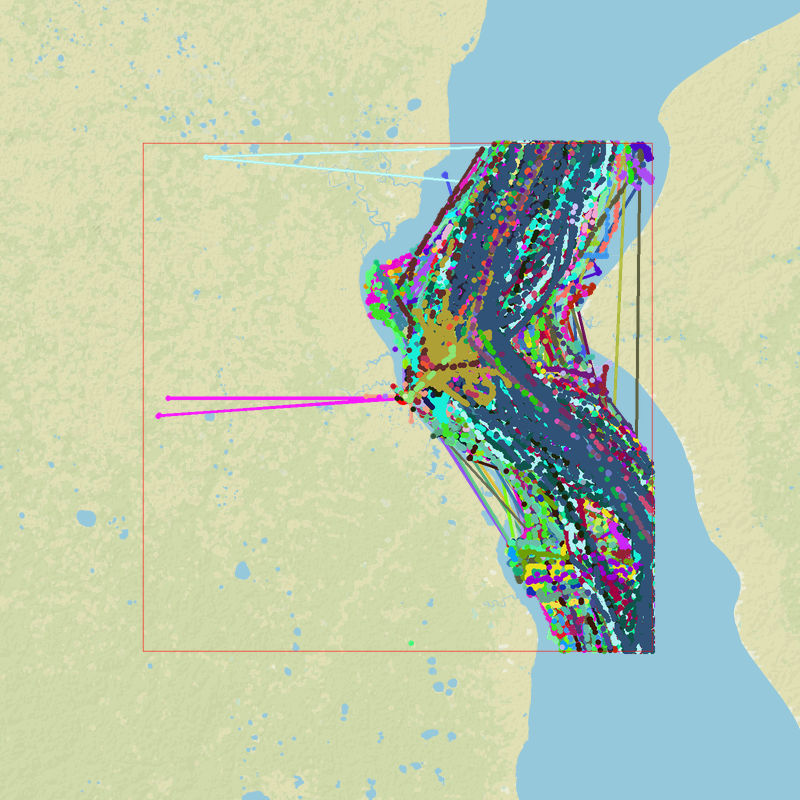
\includegraphics[width=9cm]{Images/land-points.png}
            \caption{Presence of wrong vessel coordinates on land}
        \end{figure}
        
        \end{minipage}
        
    \end{itemize}

        
    In addition, some normalization work was done on the data set.
    \\
    At the moment, all the information about the ship from which the message arrived is contained in the message record. This setting, in addition to weighing down the dataset considerably due to a huge amount of redundant data (12 fields out of 33 contain information about the ship and not the message) opens the possibility of inconsistent information.
    \\
    
    \begin{tabular}{|c|c|c|c|c|c|}
        \hline
            \textbf{index} & \textbf{imo} & \textbf{vessel\_name} & \textbf{callsign} & \textbf{vessel\_type} & \textbf{vessel\_class} \\
        \hline
            \textbf{5085} & 9120293      & KAPITAN BACHURIKHIN   & UDIZ              & Fishing               & \textcolor{red}{B}      \\
            \textbf{5086} & 9120293      & KAPITAN BACHURIKHIN   & UDIZ              & Fishing               & \textcolor{red}{A}      \\
        \hline
    \end{tabular}
    \\
    
    Above there is an example of data inconsistency messages 5085 and 5086 comes both from the same vessel but the class registered is different.
    \\
    This is impossible since the class is a vessel-related information.
    
    % PARLARE DELLA NORMALIZZAZIONE
    
    \bigbreak
    
    \begin{tabular}{|c|c|c|c|c|c|}
        \hline
            \textbf{index} & \textbf{imo} & \textbf{vessel\_name} & \textbf{callsign} & \textbf{vessel\_type} & \textbf{vessel\_class} \\
        \hline
            \textbf{31699} & 66550      & \textcolor{red}{OTA-883 *!0}   & UDIZ              & Reserved               & A      \\
            \textbf{31699} & 66550      & \textcolor{red}{OTA-883}   & UDIZ              & Reserved               & A      \\
        \hline
    \end{tabular}

\clearpage
\section{Trip Generation}

    As mentioned above, the object of analysis for anomaly detection is the entities \textbf{trips}. These are will be associated with numerical features useful for performing distance-based clustering such as DBScan. With the current state of the data, there is no deterministic way to cluster messages by trip (e.g., a trip\_id field in the message dataset).
    \\
    Therefore, it is necessary to define the concept of a trip and write an algorithm that can determine, under certain rules, to which trip each message belongs.
    \\
    The algorithm begins by sorting the receipt of messages chronologically for each ship and performs a scrolling of messages to allow grouping along the way.
    When scrolling through the messages in chronological order, the messages were associated to a trip entity. Doing that, the following factors caused it to be interrupted and a new one to be created.
    
    \begin{itemize}
    
    \item A time frame of more then \verb|SEGMENTS_MAX_DELTA_SECONDS| seconds between two consecutive messages. This variable specifies the minimum time interval between a message A and the next message B, sufficient to consider the two messages as belonging to two different trips. If this is the case, the sequence of successive messages is stopped and message B initiates a new sequence. This variable was given an arbitrary value of \textbf{86400 seconds} (24 hours)
    
    \item The arrival of a message with a change in the status of the ship to "moored". If the ship moors in a port but departs before \verb|SEGMENTS_MAX_DELTA_SECONDS| seconds have elapsed, the script considers two different trips that must be analyzed separately
    \end{itemize}
    \\
    \begin{minipage}{\linewidth}
    \begin{lstlisting}[language=Python]
coords = []
cur_coords = []
last_point = None
rows = load_vessel_file(file_path)
if len(rows) > 1:
    for row in rows:
        timestamp, latitude, longitude, status = row[0], row[1], row[2], row[3]
        # Check if is the first point
        if last_point is None:
             # check if the status is "moored"
            if status == 5:
                continue
            else:
                # register the first point
                cur_coords.append((timestamp, latitude, longitude))
        else:
            # check if the status is "moored"
            if status == 5:

                # get the last point status
                last_point_status = last_point[3]
                if last_point_status == 5:
                    pass
                else:
                    cur_coords.append((timestamp, latitude, longitude))
                    coords.append(cur_coords)
                    cur_coords = []
            else:
                delta_time = (timestamp - last_point[0])
                
                # check if the delta time is more then the max delta time
                if delta_time < settings.SEGMENTS_MAX_DELTA_TIMESTAMP_SECONDS:
                    cur_coords.append((timestamp, latitude, longitude))
                else:
                    if len(cur_coords) > 0:
                        coords.append(cur_coords)
                    cur_coords = [(timestamp, latitude, longitude)]

        last_point = (timestamp, latitude, longitude, status)
    if cur_coords:
        coords.append(cur_coords)
    \end{lstlisting}
    \end{minipage}

\section{Trip Features Association}
    One of the most important preliminary steps before applying the DBSCAN clustering method is by far the selection and computation of the \textbf{numerical features} that will become the dimensions we use to describe our entities in space.
     
    The selection of features is so important because the algorithm is able to consider trips as \textit{near} or \textit{far} from each other based on these features. Indeed, a correctly detected anomaly is one that highlights a value of some features that are substantially distant from a group of features with relatively similar values.
    
    Here are the selected trip features and how they were calculated:
    
    \subsubsection{min\_lat, max\_lat, min\_lon, max\_lon}
        These parameters are useful to describe the perimeter in which the ship moved during its voyage. Using these four features, the DBSCAN clustering algorithm can group voyages with trajectories in very similar areas.
    
    \subsubsection{start\_lat, start\_lon, end\_lat, end\_lon}
        These parameters are useful to describe the departure and arrival coordinates of the ship during the voyage. Using these four features, the DBSCAN clustering algorithm can group together voyages with similar departure and arrival points.
    
    \subsubsection{duration}
    
        This feature indicates the duration of the trip. Let \verb|ts_arr| be the array containing the timestamps of each message belonging to the trip. Duration in seconds is calculated as below:
        
        \begin{lstlisting}[language=Python]
duration = max(ts_arr) - min(ts_arr)
        \end{lstlisting}
        
    \subsubsection{delay}
    
        The delay accrued by a ship during a voyage could be a good parameter to highlight an anomaly. The latter is calculated by the presence of the parameter eta (Estimated Time of Arrival) parameter in each message. For this purpose, the first message is taken as reference, thus:
        
        \begin{lstlisting}[language=Python]
delay = trip_msgs[0]['eta'] - duration
        \end{lstlisting} 
        
        \verb|delay < 0| $\rightarrow$ the vessel is the ship is ahead of schedule;
        \\
        \verb|delay > 0| $\rightarrow$ the vessel is late.
        
    \subsubsection{mean\_sog}
    
    As explained in the Annex 1 - AIS Data Description, \textbf{sog} (Speed Over Ground) indicates the speed of the ship during its voyage. In order to point out anomalies such as excessive deceleration, this feature has been added and calculated as follows:
    
    \begin{lstlisting}[language=Python]
mean_sog = np.array([x['sog'] for x in going_msgs]).mean()
    \end{lstlisting} 
    
    Note that \verb|going_msgs| is different from \verb|trip_msgs|, as the former only considers messages in which the ship is in \textit{Under Way Using Engine} state, making the calculation of these values more meaningful.
            
    \subsubsection{mean\_cog}
    
    The message parameter \textbf{cog}, which indicates the actual direction of motion taking into account compensation for wind and other flow forces, was chosen as trip feature because the average of this value over the entire trip might reveal some anomalies in the trajectory with respect to other similar trips.
    
    \begin{lstlisting}[language=Python]
mean_sog = np.array([x['cog'] for x in going_msgs]).mean()
    \end{lstlisting} 
    
    \subsubsection{going\_time}
    The time the ship spent in the \textit{Under Way Using Engine} state during its voyage can be estimated by summing the delta time frames of each message recorded in that state compared to the immediately preceding message. If a ship has slowed down and spent less time navigating than expected, this feature can highlight that.
    
    \begin{lstlisting}[language=Python]
going_time = 0
for i, msg  in enumerate(trip_msgs):
    # The "Under Way Using Engine" has 5 as status code 
    if msg['nav_status_code'] == 5 and i < len(trip_msgs)-1:
        going_time += trip_msgs[i+1]['timestamp'] - msg['timestamp']
    \end{lstlisting} 

    
    \subsubsection{ideal\_distance}
    
    The ideal distance feature is closely related to the coordinates of the departure and arrival points. It measures the distance in kilometers as the crow flies from the departure point to the arrival point. This could be useful in figuring out if the ship took some unmotivated detour instead of going straight to the destination.
    \\
    The calculation required the use of geopy \cite{geopy} library.
    
    \begin{lstlisting}[language=Python]
ideal_distance =
    geopy.distance.distance(
        (start_lat, start_lon),
        (end_lat, end_lon)
    ).km
    \end{lstlisting} 
    
    \subsubsection{actual\_distance}
    
    The effective distance, in contrast to the previous one, measures the actual kilometers covered by the ship during its voyage. The calculation of this value is only possible by approximating the actual distance with the sum of the length of the different segments bounded by the arrival of each message.
    
    Also here the geopy \cite{geopy} library was required.
        
    \begin{lstlisting}[language=Python]
actual_distance = 0
for i, g  in enumerate(trip_msgs):
    if i < len(trip_msgs)-1:
        actual_distance += 
            geopy.distance.distance(
                (trip_msgs[i]['lat'], trip_msgs[i]['lon']),
                (trip_msgs[i+1]['lat'], trip_msgs[i+1]['lon'])
            ).km
    \end{lstlisting}

\clearpage
\section{DBSCAN Clustering}

Now that the preliminary steps are complete, we can move on to the core phase of data analysis: \clustering using the DBSCAN algorithm.
\\
Let us first describe the Python libraries that were essential for our work:
\begin{itemize}
\item \textit{numpy} \cite{numpy} which is needed for all operations based on scientific computation;
\item \textit{pandas} \cite{pandas} which is a pillar for data analysis and manipulation;
\item \textit{scikit learn} \cite{sklearn} which provides several easy-to-implement machine learning tools;
\item \textit{matplotlib} \cite{matplotlib} and \textit{seaborn} \cite{seaborn} for data visualization.
\end{itemize}

Let \verb|df| (\textit{DataFrame}) be the container of all previously computed features. A table-like structure where each row is a trip and the columns are represented by the selected features.

\begin{table}[H]
\centering
\begin{tabular}{|l|l|l|l|l|l|l|l|l|l|}
\hline
\textbf{min lat}  & \textbf{max lat}  & \textbf{...}  & \textbf{delay}     & \textbf{mean sog} & \textbf{mean cog}  & \textbf{going time} & \textbf{ideal dist}  \\
\hline
66.640 & 66.648 & ... & 9038337 & 0.227  & 218.476 & 83663 & 9.157         \\
68.117 & 73.138 & ... & 8949470 & 8.025  & 128.487 & 172530 & 533.221       \\
66.629 & 67.830 & ... & 9036649 & 3.527  & 147.169 & 85351 & 135.627       \\
72.544 & 72.779 & ... & 9213950 & 7.296  & 103.688 & 28050 & 95.251        \\
66.640 & 68.098 & ... & 9036361 & 4.382  & 89.9779 & 85639 & 167.403      \\
\hline
\end{tabular}
\caption{Example of trip features dataframe}
\end{table}

\subsection{Trip features correlation Analysis}

This phase begins with the calculation of the correlation matrix. Using the Pearson correlation index \verb|[-1,1]|, we can see how much the variables explain each other, or more precisely, how strongly one variable is correlated with another.

A correlation of 1 indicates that two variables are perfectly correlated, while a correlation of -1 indicates that two variables are inversely correlated. Values close to 0 indicate that the two variables are not correlated at all.

\begin{lstlisting}[language=Python]
df.corr()
\end{lstlisting}

In addition a heatmap to interpret the \textbf{correlation matrix} more quickly was used.

\begin{figure}[H]
    \centering
    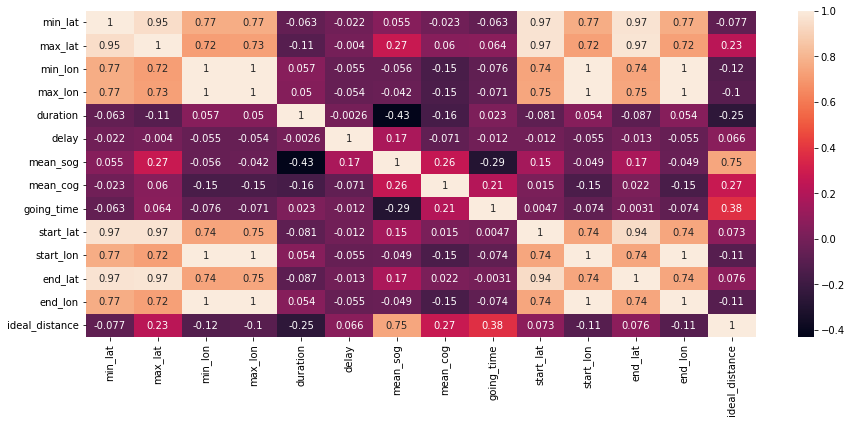
\includegraphics[width=17cm]{Images/1/heatmap.png}
    \caption{Example of trip features correlation heatmap}
\end{figure}

After doing this, we can plot graphs to highlight the correlation between some features

We can immediately say that the variables \textbf{end\_lat} and \textbf{max\_lat} are strongly correlated (correlation close to 1), as well as for all coordinate pairs.

In contrast \textbf{mean\_sog} and \textbf{duration} are slightly inversely correlated (correlation less than 0).

In contrast, variables such as \textbf{end\_lat} and \textbf{mean\_cog} are weakly correlated (correlation close to 0).

We visualize these pairs of variables through \textbf{scatterplots} to confirm what we observed:

\begin{figure}[H]
    \centering
    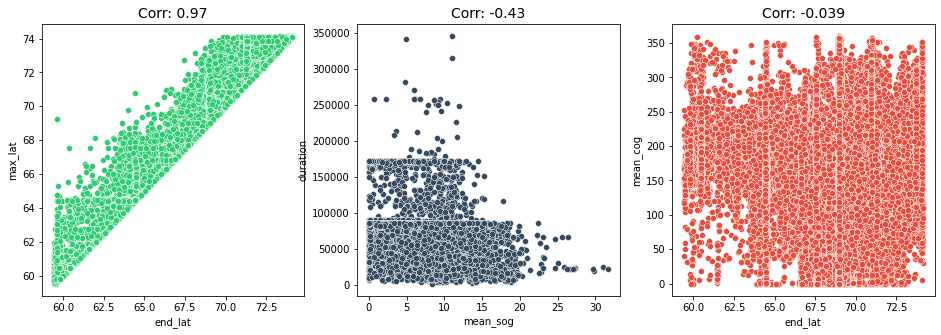
\includegraphics[width=16cm]{Images/1/scatterplots.png}
    \caption{Example of scatterplots with strongly, inversely and weakly correlated features}
\end{figure}

\subsection{Trip features standardization}

In order to further clean our data before core processing in the clustering phase, this methodology includes removing rows with missing values, i.e., trips that do not contain enough information to compute some features.

After that, a necessary step is the standardization of the data set to avoid problems related to the different scaling of variables in practice.

\textbf{Boxplots} are charts that allow us to visualize the distribution of several variables at the same time, in order to verify they are all on the same scale after the normalization.

\begin{lstlisting}[language=Python]
cleaned_df = df.dropna()
scaler = StandardScaler()
scaled_array = scaler.fit_transform(cleaned_df)
scaled_df = pd.DataFrame( scaled_array, columns = cleaned_df.columns )
\end{lstlisting}

\begin{figure}[H]
    \centering
    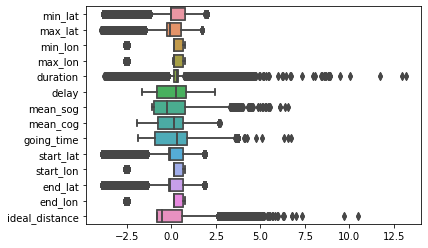
\includegraphics[width=16cm]{Images/1/boxplot.png}
    \caption{Example of boxplot of the trip features after standardization}
\end{figure}


\subsection{DBSCAN implementation}
The DBSCAN is a clustering algorithm that belongs to the category of so-called density-based algorithms, since it only identifies regions of the feature space where the density of points (or observations) is greater.

All observations that are close to each other are grouped into a cluster. Those that appear isolated are referred to as noise.

As mentioned earlier the DBSCAN needs two \textbf{parameters}:

\begin{itemize}
\item $\varepsilon$ which corresponds to the distance within which to search for neighboring points;
\item \textit{n} which corresponds to the minimum number of points in order to compose a cluster.
\end{itemize}

For the sake of brevity we can say that the DBSCAN does nothing more than search for all those clusters whose points are greater than or equal to a number less than $\varepsilon$.

Just as very first step, we give the two parameters an arbitrary value and analyze the results by measuring the number of clusters and the significance of outliers during the hyperparameter phase.

\begin{lstlisting}[language=Python]
dbscan_model = DBSCAN(eps = 0.75, min_samples = 5)
dbscan_model.fit(scaled_df)
\end{lstlisting}

The DBSCAN clustering algorithm has been implemented and within \verb|dbscan_model| we will find all the information regarding the clusters created and the trips considered as \textbf{outliers}. In the testing chapter, we will take a more in-depth look at how to reveal from outliers by applying this methodology to a real data set.

\subsection{Searching for hyperparameters}

Since DBSCAN is an unsupervised model it does not enjoy any metrics to calculate its accuracy.

This chapter is only about understanding how to perform the search for hyperparameters, and then explain how the correct parameters were selected in the chapter on testing.
This requires observing how the metrics change as a function of selected hyperparameters. We define the hyperparameters set to be tested:

\begin{lstlisting}[language=Python]
eps_to_test = [round(eps,1) for eps in np.arange(0.1, 2, 0.1)]
min_samples_to_test = range(5, 50, 5)

print("EPS:", eps_to_test)
print("MIN_SAMPLES:", list(min_samples_to_test))
\end{lstlisting}


\begin{minipage}{\linewidth}
\begin{lstlisting}[language=Python]
iter = 0
for eps in eps_to_test:
    for min_samples in min_samples_to_test:
        
        iter += 1

        # Calculating the metrics
        noise_metric, cluster_metric = get_metrics(eps, min_samples, scaled_df, iter_)
\end{lstlisting}
\end{minipage}



\chapter{Testing}
\label{ch:testing}

\section{Overview}

This chapter describes the implementation of the \ref{ch:methodology} chapter's methodology through the usage and analysis of a data set provided by Arcos \cite{arcos}. 



- descrizione dei dati originali, percentuali
- descrizione dei viaggi, percentuali
- heatmap
- 

\subsection{The original Dataset}
The source dataset selected to carry out testing of the described methodology is as mentioned composed of AIS messages.
Nel dettaglio, si tratta di messaggi provenienti da navi che hanno attraversato la zona artica e dintorni negli anni 2019, 2020 e 2021.
In numbers:
\begin{itemize}
\item 95,294,750 AIS messages;
\item 10,058 different vessels;
\item 6,777 segments generated.
\end{itemize}


\subsection{PCA, a graphical clusters rapresentation technique}

In order to a get an idea of the clusters from a graphical point of view, a \textbf{dimensionality reduction} procedure was used: \textbf{Principal Component Analysis}.
PCA has the task of reducing an input space with n dimensions into a space with smaller number of dimensions.
Since the goal in this case was to obtain a graphical representation of the clusters, the number of components to which the 7 input components were reduced was \textbf{2}.

What DBSCAN produces in this context is a dataset of clusters and all the possible information to locate in a 7-dimensional space (the 7 chosen features, indeed) the trips that were given to it as input.
More precisely, each pathway is classified as:
\begin{itemize}
\item \textbf{Core Point} if it is a point that contributed to the cluster expansion, as described in the section; \ref{subsec:dbscan-example}
\item \textbf{Non-Core Point} if it is a point that has not contributed to cluster expansion;
\item \textbf{Outlier} if for some reason the algorithm did not include the trip in any generated cluster.
\end{itemize}

Of course, it is very complicated to depict a space with a number of dimensions greater than 2, so the result of this DBSCAN would be difficult to represent.

Using the Principal Component Analysis (PCA) technique with two components, it has been possible to graphically represent the obtained clusters despite the 7-dimensions space of the original data.

\begin{figure}[H]
    \centering
    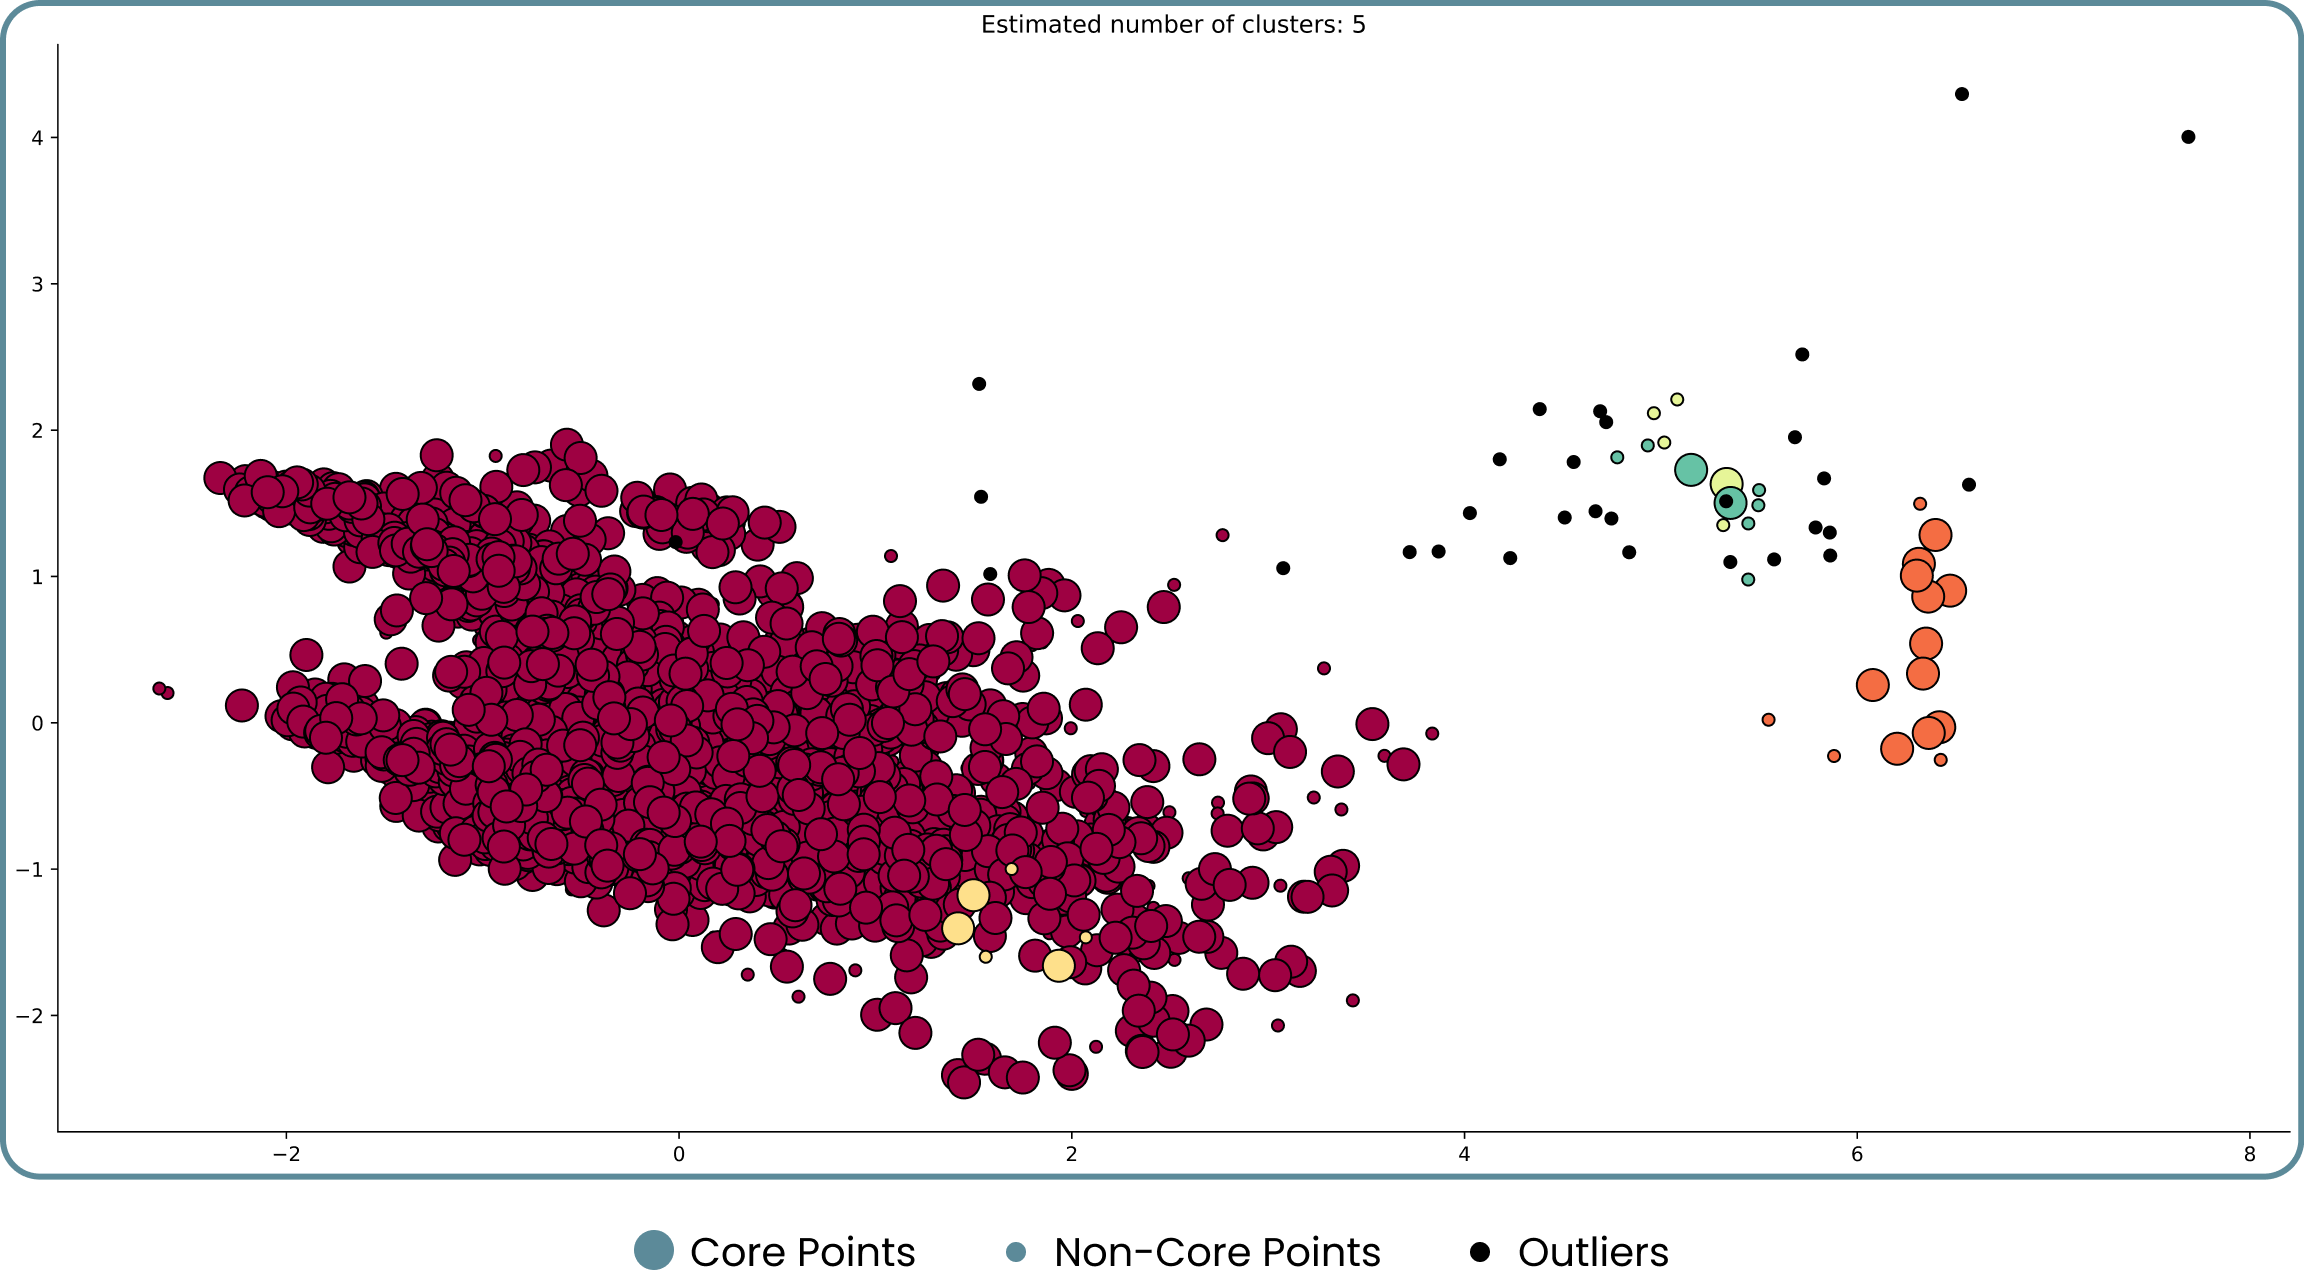
\includegraphics[width=13cm]{Images/3/clusters.png}
    \caption{Graphic representation of clusters in 2 components with PCA}
    
    
\end{figure}


\chapter{Conclusions and future developments}
\label{ch:conclusions}%
A final chapter containing the main conclusions of your research/study
and possible future developments of your work have to be inserted in this chapter.
    
%-------------------------------------------------------------------------
%	BIBLIOGRAPHY
%-------------------------------------------------------------------------

\addtocontents{toc}{\vspace{2em}} % Add a gap in the Contents, for aesthetics
\bibliography{Thesis_bibliography} % The references information are stored in the file named "Thesis_bibliography.bib"

%-------------------------------------------------------------------------
%	APPENDICES
%-------------------------------------------------------------------------

\cleardoublepage
\addtocontents{toc}{\vspace{2em}} % Add a gap in the Contents, for aesthetics
\appendix

\chapter{Appendix A - AIS Data Description}
\label{app:data-description}
In addition to the information required by the AIS standard, message data enriched with more information was used for the purpose of this thesis.
    
The fields of the original source AIS data of single entry (that represents a message) are described below.

\subsubsection{FID}
    The FID is the unique message identifier expressed as v4 UUID.
\subsubsection{MMSI}
    The \textbf{Maritime Mobile Service Identity} (MMSI) is a nine-digit number identifying the vessel or boat. Since it is always present is the field that is most frequently used to identify a vessel
\subsubsection{IMO}
    \textbf{IMO} stands for International Maritime Organization and it is another way to uniquely indentify a vessel or boat. Not all means of maritime transport comply to this standard and which is why some of the AIS messages do not have this field.
\subsubsection{Vessel Name}
    Name of the vessel.
\subsubsection{Callsign}
    A Call Sign is a unique identifier for a transmitter station on the boat. Of course, since a vessel can be equipped by more than one radio station, and since these stations can be interchanged between ships, there is no static correlation between call sign and ship.
\subsubsection{Vessel Type}
    This field describe a type of vessel based on a first classification: the purpose of the ship. \\
    Possible options: 'Tanker' 'Tug' 'Fishing' 'Other' 'Reserved' 'Cargo' 'Unknown' 'Dredging' 'Not Available' 'Military' 'SAR' 'HSC' 'Pilot' 'Towing' 'Vessel With Anti-Pollution Equipment' 'Diving' 'Port Tender' 'Pleasure Craft' 'Law Enforcement' 'Passenger' 'WIG' 'Sailing' 'Ships Not Party to Armed Conflict' 'Spare' 'Medical Transport'
\subsubsection{Vessel Type Code}
    Numeric version of the previous field.
\subsubsection{Vessel Type Cargo}
    Notes about cargo, if present.
\subsubsection{Vessel Class}
    Here is the class of vessel that help quantify the degree of seaworthiness of a boat based on the wave height and wind speed for which the boat is designed.\cite{vessel_classes}
    
    \begin{itemize}
    \item Category A: Ocean;
    \item Category B: Offshore;
    \item Category C: InShore;
    \item Category D: Inland or sheltered coastal waters.
    \end{itemize}

    
\subsubsection{Length}
    Length of vessel, in meters.
\subsubsection{width}
    Width of vessel, in meters.
\subsubsection{Flag Country}
    Country name of vessel flag.
\subsubsection{Flag Code}
    Country code of vessel flag.
\subsubsection{Destination}
    Destination of the trip of which the message is a part.
\subsubsection{ETA}
    This numeric field contains the Estimated Time of Arrival, expressed as the remaining estimated milliseconds to arrive at the destination.
\subsubsection{Draught}
    The Draught of a vessel measures the maximum depth of any part of the vessel respect of the waterline, in meters. This determines the minimum depth of water a ship or boat can safely navigate. In some applications of analyzing these data, this value could be used as a proxy for the ship's cargo weight.
\subsubsection{Longitude}
    The current longitude according to the geographic coordinate system of the vessel.
\subsubsection{Latitude}
    The current latitude according to the geographic coordinate system of the vessel.
\subsubsection{SOG}
    Speed over Ground (SOG) is the speed of the vessel in one hour with respect to the land or any other fixed object such as buoys.
\subsubsection{COG}
    The Course Over Ground is the actual direction in degree of the motion considering the compensation for wind and current forces by changing the actual heading of the boat.
\subsubsection{ROT}
    Rate of turn indicator, indicates the rate a ship is turning in degrees per minute (°/min).
\subsubsection{Heading}
    The heading of a ship is a parameter similar to COG, since it too measures the direction of a ship. The heading is the compass direction the boat is pointing, and it may not match COG if there are current and tidal effects. Heading is instantaneous, COG can be derived from boat's motion over time.
    \\
    \begin{center}
    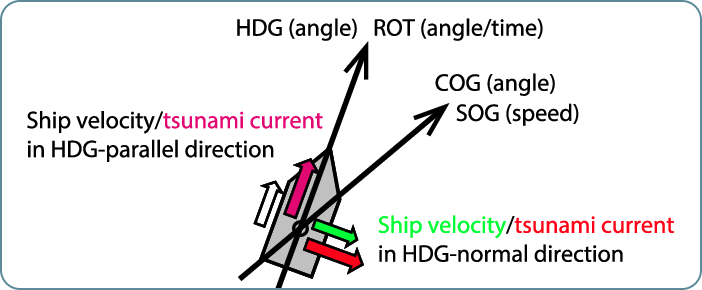
\includegraphics[width=10cm]{Images/appendices/cog-sog.png}
    \end{center}
\subsubsection{Nav Status}
    The status of the vessel. Possible options: \\'Under Way Using Engine' 'Engaged In Fishing' 'Not Defined' 'At Anchor' 'Restricted Manoeuvrability' 'Moored' 'Underway Sailing' 'Unknown' 'Not Under Command'.
\subsubsection{Nav Status Code}
    The status code of the vessel, related to the previous field.
\subsubsection{Source}
    This field describe the source of the message. The possible options are S-AIS and T-AIS.
    S-AIS stands for Satellite-based AIS.
    T-AIS stands for Terrestrial-based AIS.
\subsubsection{TS POS UTC}
    Datetime position in the format \verb|YYYYMMDDHHIISS|
\subsubsection{TS Static UTC}
    Datetime static in the format \verb|YYYYMMDDHHIISS|
\subsubsection{DT POS UTC}
    Datetime position in the format \verb|YYYY-MM-DD HH:II:SS|
\subsubsection{DT Static UTC}
    Datetime static in the format \verb|YYYY-MM-DD HH:II:SS|
\subsubsection{Vessel Type Main}
    Category of vessel. Possible options:\\ 'Oil And Chemical Tanker' 'Fishing Vessel' 'General Cargo Ship' 'Bulk Carrier' 'Gas Tanker' 'Tug' 'Service Ship' 'Offshore Vessel' 'Passenger Ship' 'Specialized Cargo Ship' 'Other' 'Pleasure Craft' 'Other Tanker'.
\subsubsection{Vessel Type Sub}
    Subcategory of vessel. Possible options:\\ 'Crude Oil Tanker' nan 'Lng Tanker' 'Pusher Tug' 'Research Vessel' 'Offshore Tug Supply Ship' 'Hopper Dredger' 'Refrigerated Cargo Ship' 'Dredger' 'Utility Vessel' 'Chemical Oil Products Tanker' 'Oil Products Tanker' 'Cruise Ship' 'Crane Ship' 'Icebreaker' 'Offshore Support Vessel' 'Nuclear Fuel Carrier' 'Landing Craft' 'Sailing Vessel' 'Patrol Vessel' 'Fish Carrier' 'Salvage Ship' 'Drilling Ship' 'Fish Factory Ship' 'Chemical Tanker' 'Fishing Support Vessel' 'Live Fish Carrier' 'Asphalt Bitumen Tanker'.
\subsubsection{Message Type}
    A numeric code that identifies the message type.

\chapter{Appendix B - Testing Results}
\label{app:tessting-results}

\section*{Cluster \#1}
Model Accuracy: 0.9003


\begin{tabular}{llrrlll}
 & Feature & Importance & Sign & AVG outliers & AVG non outliers & T-test p value \\
0 & going\_time\_perc & 0.041309 & 1 & 58.15 & 84.27 & 8.19e-23 \\
1 & var\_coeff\_draught & 0.024866 & -1 & 504.5 & 0.9957 & 3.32e-71 \\
2 & mean\_cog & 0.012223 & 1 & 138.9 & 157.9 & 5.16e-03 \\
3 & rel\_delay & 0.008588 & -1 & 603.5 & 149.6 & 9.03e-81 \\
4 & extra\_distance & 0.007406 & -1 & 196.0 & 102.8 & 1.53e-13 \\
5 & mean\_sog & 0.003031 & 1 & 3.718 & 8.646 & 4.78e-34 \\
6 & duration & 0.000001 & -1 & 3.214e+06 & 2.404e+05 & 1.36e-252 \\
\end{tabular}



\section*{Cluster \#2}
Model Accuracy: 0.9189


\begin{tabular}{llrrlll}
 & Feature & Importance & Sign & AVG outliers & AVG non outliers & T-test p value \\
0 & var\_coeff\_draught & 0.067669 & -1 & 504.5 & 0.6771 & 1.07e-01 \\
1 & rel\_delay & 0.062380 & -1 & 603.5 & -0.7285 & 7.07e-03 \\
2 & extra\_distance & 0.023852 & -1 & 196.0 & 67.24 & 3.32e-03 \\
3 & mean\_cog & 0.010328 & -1 & 138.9 & 139.3 & 9.83e-01 \\
4 & going\_time\_perc & 0.007141 & -1 & 58.15 & 0.0 & 3.21e-09 \\
5 & mean\_sog & 0.000406 & -1 & 3.718 & 0.02249 & 1.45e-03 \\
6 & duration & 0.000001 & 1 & 3.214e+06 & 9.567e+06 & 2.39e-14 \\
\end{tabular}



\section*{Cluster \#3}
Model Accuracy: 0.8649


\begin{tabular}{llrrlll}
 & Feature & Importance & Sign & AVG outliers & AVG non outliers & T-test p value \\
0 & var\_coeff\_draught & 0.032755 & -1 & 504.5 & 1.608 & 1.07e-01 \\
1 & rel\_delay & 0.030176 & -1 & 603.5 & -0.7303 & 7.07e-03 \\
2 & extra\_distance & 0.009722 & -1 & 196.0 & 153.5 & 3.35e-01 \\
3 & mean\_cog & 0.004040 & -1 & 138.9 & 177.1 & 3.88e-02 \\
4 & going\_time\_perc & 0.001097 & -1 & 58.15 & 97.17 & 4.71e-05 \\
5 & mean\_sog & 0.000196 & -1 & 3.718 & 0.03656 & 1.52e-03 \\
6 & duration & 0.000000 & 1 & 3.214e+06 & 9.753e+06 & 5.06e-15 \\
\end{tabular}



\section*{Cluster \#4}
Model Accuracy: 0.8182


\begin{tabular}{llrrlll}
 & Feature & Importance & Sign & AVG outliers & AVG non outliers & T-test p value \\
0 & var\_coeff\_draught & 0.233151 & -1 & 504.5 & 1.151e-14 & 3.92e-01 \\
1 & going\_time\_perc & 0.222628 & 1 & 58.15 & 100.0 & 1.89e-02 \\
2 & mean\_sog & 0.165244 & -1 & 3.718 & 6.457 & 2.07e-01 \\
3 & extra\_distance & 0.057045 & 1 & 196.0 & 5.968 & 2.09e-02 \\
4 & mean\_cog & 0.021663 & -1 & 138.9 & 124.3 & 6.61e-01 \\
5 & rel\_delay & 0.005435 & -1 & 603.5 & 1.498e+03 & 3.45e-02 \\
6 & duration & 0.001325 & -1 & 3.214e+06 & 6.746e+03 & 2.78e-02 \\
\end{tabular}



\section*{Cluster \#5}
Model Accuracy: 0.9091


\begin{tabular}{llrrlll}
 & Feature & Importance & Sign & AVG outliers & AVG non outliers & T-test p value \\
0 & mean\_sog & 1.606796 & 1 & 3.718 & 9.1 & 3.69e-02 \\
1 & extra\_distance & 0.968915 & -1 & 196.0 & 1.096 & 4.49e-02 \\
2 & going\_time\_perc & 0.436247 & 1 & 58.15 & 100.0 & 4.67e-02 \\
3 & mean\_cog & 0.090936 & -1 & 138.9 & 65.99 & 6.63e-02 \\
4 & rel\_delay & 0.007929 & -1 & 603.5 & 2.044e+03 & 4.23e-03 \\
5 & var\_coeff\_draught & 0.006835 & -1 & 504.5 & 1.047e-14 & 4.69e-01 \\
6 & duration & 0.005733 & -1 & 3.214e+06 & 4.819e+03 & 6.23e-02 \\
\end{tabular}



% LIST OF FIGURES
\listoffigures

% LIST OF TABLES
\listoftables

% ACKNOWLEDGEMENTS

\chapter*{Acknowledgements}



\cleardoublepage

\end{document}
